\documentclass{scrreprt}

\usepackage[english,ngerman]{babel} 
\usepackage[utf8]{inputenc} 
\usepackage{graphicx}
\usepackage{dsfont}
\usepackage{amsmath}

\setcounter{MaxMatrixCols}{20}

\title{TH1 - Aufgabenblatt 2}
\author{Andreas Krohn, Erik Andresen, Benjamin Vetter, Andreas Basener}

\begin{document}

\maketitle

\begin{enumerate}

\item Welche Eigenschaften sollte Eure Gleisanlage haben? (informelle Beschreibung)

\begin{itemize}
  \item Deadlock-Freiheit
  \item Starvation-Frei
  \item Beschränkt bzgl. der maximalen Anzahl an fahrenden Zügen pro Gleisabschnitt
  \item Kollisionsfrei
  \item Alpenpanorama
\end{itemize}

\newpage

\item Modellierung:

(a) Modelliert die einzelnen o.g. Gleise, Weichen und die Schranke jeweils mit
    einem eigenen S/T-Netz. Wie werden die Züge darin modelliert?


Ein Gleis ist eine Stelle mit maximaler Belegung von eins. Wenn ein Zug dieses Gleis belegt befindet sich auf der Stelle ein Token.
Die Weichen werden über zwei alternative Transitionen, die von der Stelle weglaufen modelliert: Pro Weiche und Richtung existiert eine Transition, d.h. über das Schalten der
jeweiligen Transition wird gewählt wie der Zug weiterfahren soll.

Der Bahnübergang ist eine Transition auf der Bahnstrecke zwischen zwei Gleisabschnitten (Stellen), die nur schaltet wenn sich niemand auf dem Bahnübergang befindet (Token auf Bahnübergang frei). Wird der Bahnübergang (Bü) betreten befindet sich kein Token mehr auf "`Bahnübergang frei"' und damit kann der Zug den Bahnübergang nicht passieren.

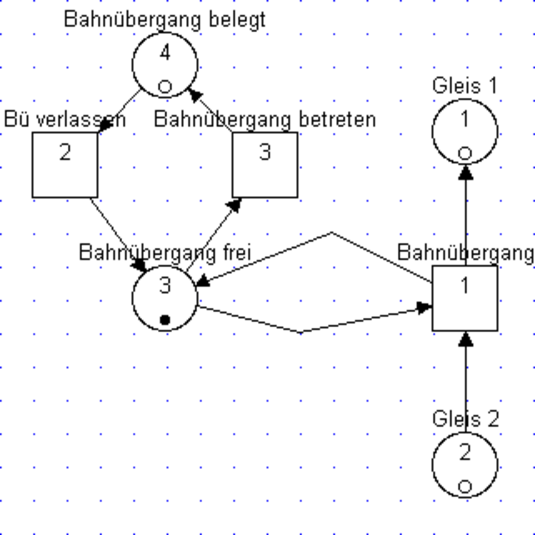
\includegraphics[width=0.45\textwidth]{bahnuebergang.pdf}

(b) Setzt die einzelnen S/T-Netze zusammen, so dass mind. jedes Gleis, jede Weiche und die Schranke einmal in Eurer Gleisanlage vorhanden sind und gebt eine Anfangsmarkierung mit zwei Zügen an.

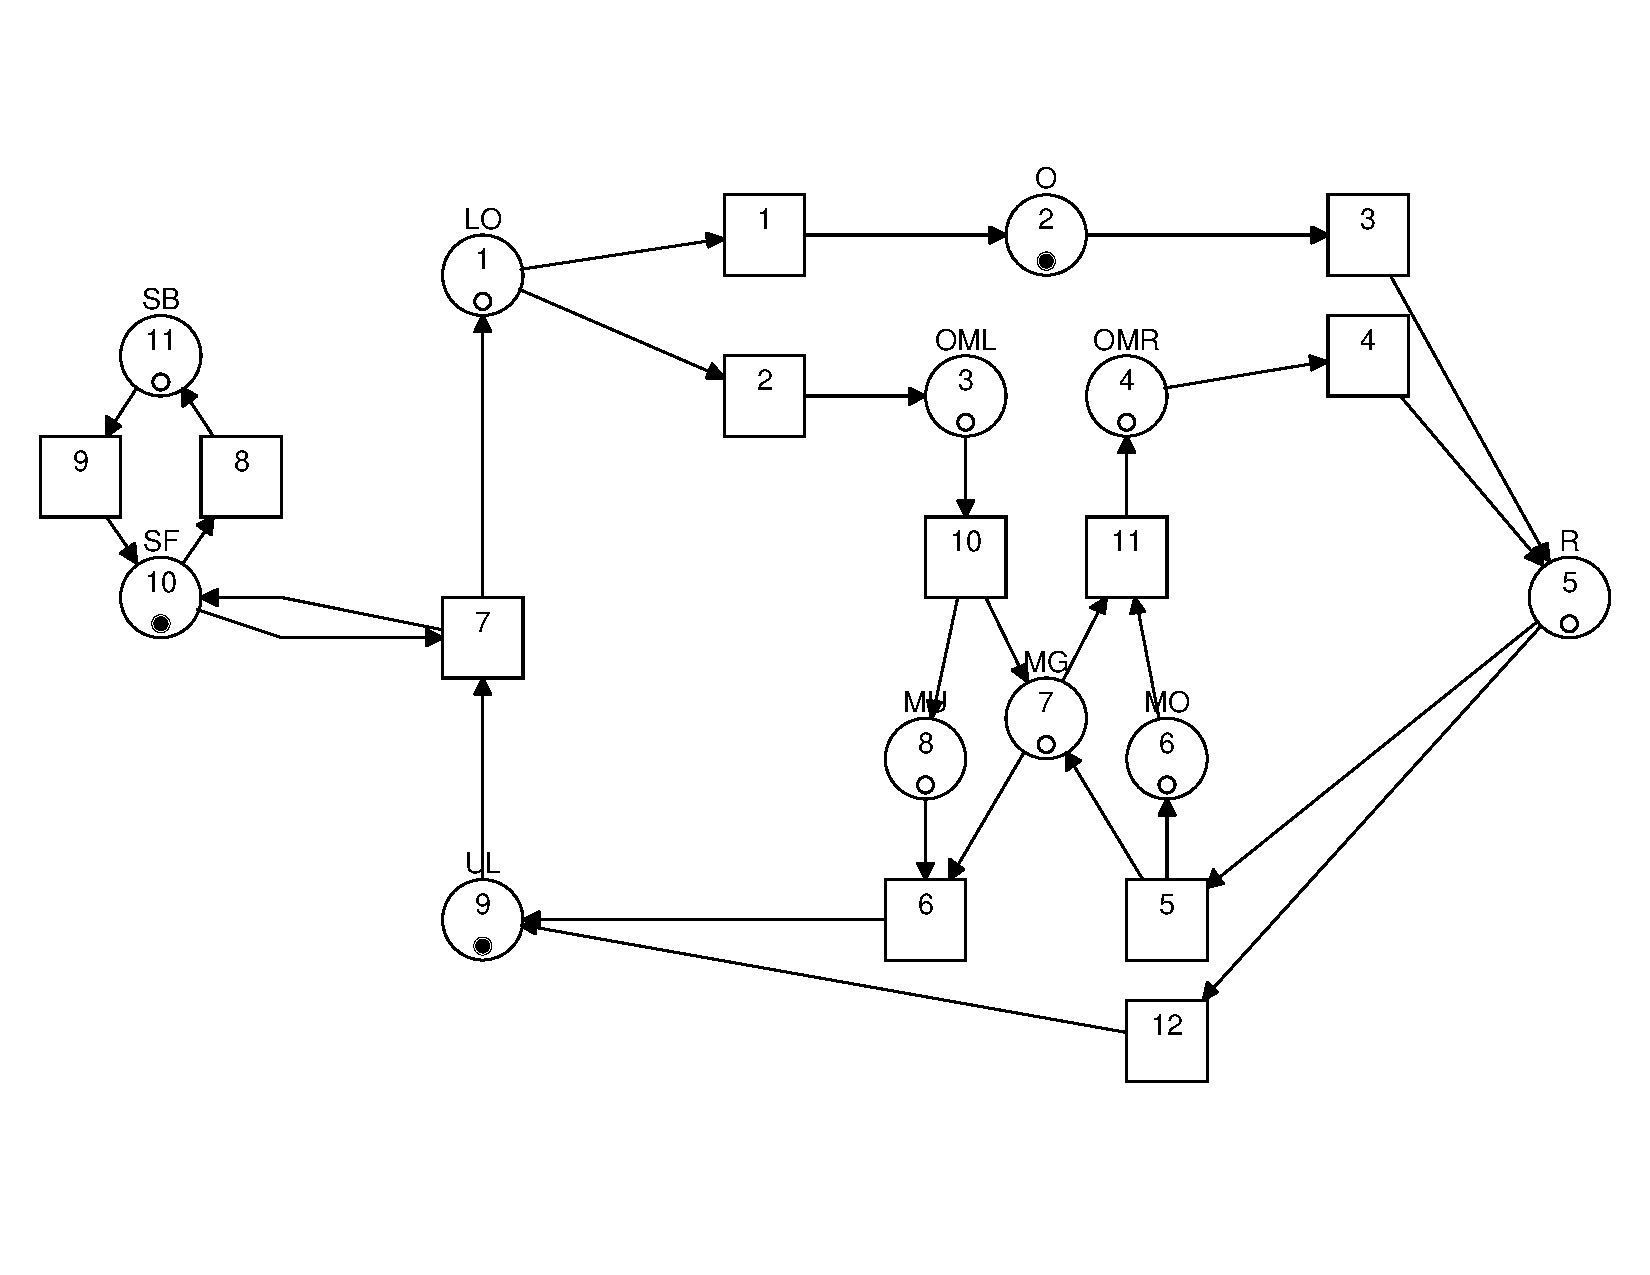
\includegraphics[width=1\textwidth]{prak2_aufg2.pdf}

\item Analyse:

(a) Berechnet die P-Invarianten Euer Gleisanlage.

\begin{enumerate}
\item S/T-Netz in Matrixdarstellung:

\( P = \{LO, O, OML, OMR, R, MU, MG, MO, UL, SB, SF\} \)

\(LO < O < OML < OMR < R < MU < MG < MO < UL < SB < SF\)

\( T = \{T1, T2, T3, T4, T5, T6, T7, T8, T9, T10, T11, T12\} \)

\( \underline{post} = \begin{pmatrix}
% 1 & 2 & 3 & 4 & 5 & 6 & 7 & 8 & 9 & A & B & C \\
0 & 0 & 0 & 0 & 0 & 0 & 1 & 0 & 0 & 0 & 0 & 0 \\ % LO
1 & 0 & 0 & 0 & 0 & 0 & 0 & 0 & 0 & 0 & 0 & 0 \\ % O
0 & 1 & 0 & 0 & 0 & 0 & 0 & 0 & 0 & 0 & 0 & 0 \\ % OML
0 & 0 & 0 & 0 & 0 & 0 & 0 & 0 & 0 & 0 & 1 & 0 \\ % OMR
0 & 0 & 1 & 1 & 0 & 0 & 0 & 0 & 0 & 0 & 0 & 0 \\ % R
0 & 0 & 0 & 0 & 0 & 0 & 0 & 0 & 0 & 1 & 0 & 0 \\ % MU
0 & 0 & 0 & 0 & 1 & 0 & 0 & 0 & 0 & 0 & 0 & 0 \\ % MG
0 & 0 & 0 & 0 & 1 & 0 & 0 & 0 & 0 & 0 & 0 & 0 \\ % MO
0 & 0 & 0 & 0 & 0 & 1 & 0 & 0 & 0 & 0 & 0 & 1 \\ % UL
0 & 0 & 0 & 0 & 0 & 0 & 0 & 1 & 0 & 0 & 0 & 0 \\ % SB
0 & 0 & 0 & 0 & 0 & 0 & 1 & 0 & 1 & 0 & 0 & 0 \\ % SF
\end{pmatrix}\)

\( \underline{pre} = \begin{pmatrix}
% 1 & 2 & 3 & 4 & 5 & 6 & 7 & 8 & 9 & A & B & C \\
1 & 1 & 0 & 0 & 0 & 0 & 0 & 0 & 0 & 0 & 0 & 0 \\ % LO
0 & 0 & 1 & 0 & 0 & 0 & 0 & 0 & 0 & 0 & 0 & 0 \\ % O
0 & 0 & 0 & 0 & 0 & 0 & 0 & 0 & 0 & 1 & 0 & 0 \\ % OML
0 & 0 & 0 & 1 & 0 & 0 & 0 & 0 & 0 & 0 & 0 & 0 \\ % OMR
0 & 0 & 0 & 0 & 1 & 0 & 0 & 0 & 0 & 0 & 0 & 1 \\ % R
0 & 0 & 0 & 0 & 0 & 1 & 0 & 0 & 0 & 0 & 0 & 0 \\ % MU
0 & 0 & 0 & 0 & 0 & 1 & 0 & 0 & 0 & 0 & 1 & 0 \\ % MG
0 & 0 & 0 & 0 & 0 & 0 & 0 & 0 & 0 & 0 & 1 & 0 \\ % MO
0 & 0 & 0 & 0 & 0 & 0 & 1 & 0 & 0 & 0 & 0 & 0 \\ % UL
0 & 0 & 0 & 0 & 0 & 0 & 0 & 0 & 1 & 0 & 0 & 0 \\ % SB
0 & 0 & 0 & 0 & 0 & 0 & 1 & 1 & 0 & 0 & 0 & 0 \\ % SF
\end{pmatrix}\)

\( \underline{N} = (P, T, \underline{pre}, \underline{post})\)

\( \underline{I} = \underline{post} - \underline{pre} = \begin{pmatrix}
% 1 & 2 & 3 & 4 & 5 & 6 & 7 & 8 & 9 & A & B & C \\
-1 &-1 & 0 & 0 & 0 & 0 & 1 & 0 & 0 & 0 & 0 & 0 \\ % LO
 1 & 0 &-1 & 0 & 0 & 0 & 0 & 0 & 0 & 0 & 0 & 0 \\ % O
 0 & 1 & 0 & 0 & 0 & 0 & 0 & 0 & 0 &-1 & 0 & 0 \\ % OML
 0 & 0 & 0 &-1 & 0 & 0 & 0 & 0 & 0 & 0 & 1 & 0 \\ % OMR
 0 & 0 & 1 & 1 &-1 & 0 & 0 & 0 & 0 & 0 & 0 &-1 \\ % R
 0 & 0 & 0 & 0 & 0 &-1 & 0 & 0 & 0 & 1 & 0 & 0 \\ % MU
 0 & 0 & 0 & 0 & 1 &-1 & 0 & 0 & 0 & 0 &-1 & 0 \\ % MG
 0 & 0 & 0 & 0 & 1 & 0 & 0 & 0 & 0 & 0 &-1 & 0 \\ % MO
 0 & 0 & 0 & 0 & 0 & 1 &-1 & 0 & 0 & 0 & 0 & 1 \\ % UL
 0 & 0 & 0 & 0 & 0 & 0 & 0 & 1 &-1 & 0 & 0 & 0 \\ % SB
 0 & 0 & 0 & 0 & 0 & 0 & 0 &-1 & 1 & 0 & 0 & 0 \\ % SF
\end{pmatrix} \)

\( M_0 = \begin{pmatrix}
0 \\ % LO
1 \\ % O
0 \\ % OML
0 \\ % OMR
0 \\ % R
0 \\ % MU
0 \\ % MG
0 \\ % MO
1 \\ % UL
0 \\ % SB
1 \\ % SF
\end{pmatrix} \)

\item Lösung des Gleichungssystems \( \underline{I}^T * x = \underline{0} \)

\( \begin{pmatrix}
-1 & 1 & 0 & 0 & 0 & 0 & 0 & 0 & 0 & 0 & 0  \\
-1 & 0 & 1 & 0 & 0 & 0 & 0 & 0 & 0 & 0 & 0  \\
 0 &-1 & 0 & 0 & 1 & 0 & 0 & 0 & 0 & 0 & 0  \\
 0 & 0 & 0 &-1 & 1 & 0 & 0 & 0 & 0 & 0 & 0  \\
 0 & 0 & 0 & 0 &-1 & 0 & 1 & 1 & 0 & 0 & 0  \\
 0 & 0 & 0 & 0 & 0 &-1 &-1 & 0 & 1 & 0 & 0  \\
 1 & 0 & 0 & 0 & 0 & 0 & 0 & 0 &-1 & 0 & 0  \\
 0 & 0 & 0 & 0 & 0 & 0 & 0 & 0 & 0 & 1 &-1  \\
 0 & 0 & 0 & 0 & 0 & 0 & 0 & 0 & 0 &-1 & 1  \\
 0 & 0 &-1 & 0 & 0 & 1 & 0 & 0 & 0 & 0 & 0  \\
 0 & 0 & 0 & 1 & 0 & 0 &-1 &-1 & 0 & 0 & 0  \\
 0 & 0 & 0 & 0 &-1 & 0 & 0 & 0 & 1 & 0 & 0  \\
\end{pmatrix} * x = \underline{0}\)

% TODO ggf. Gleichungssystem manuell lösen

$I_{P_1} = (1, 1, 1, 1, 1, 0, 1, 0, 1, 0, 0)^T$

$I_{P_2} = (0, 0, 0, 0, 0, 0, 0, 0, 0, 1, 1)^T$

$I_{P_3} = (1, 1, 1, 1, 1, 1, 0, 1, 1, 0, 0)^T$

\end{enumerate}

(b) Berechnet die T-Invarianten Euer Gleisanlage.

Lösung des Gleichungssystems \( \underline{I} * x = \underline{0} \):

\( \begin{pmatrix}
-1 &-1 & 0 & 0 & 0 & 0 & 1 & 0 & 0 & 0 & 0 & 0 \\
 1 & 0 &-1 & 0 & 0 & 0 & 0 & 0 & 0 & 0 & 0 & 0 \\
 0 & 1 & 0 & 0 & 0 & 0 & 0 & 0 & 0 &-1 & 0 & 0 \\
 0 & 0 & 0 &-1 & 0 & 0 & 0 & 0 & 0 & 0 & 1 & 0 \\
 0 & 0 & 1 & 1 &-1 & 0 & 0 & 0 & 0 & 0 & 0 &-1 \\
 0 & 0 & 0 & 0 & 0 &-1 & 0 & 0 & 0 & 1 & 0 & 0 \\
 0 & 0 & 0 & 0 & 1 &-1 & 0 & 0 & 0 & 0 &-1 & 0 \\
 0 & 0 & 0 & 0 & 1 & 0 & 0 & 0 & 0 & 0 &-1 & 0 \\
 0 & 0 & 0 & 0 & 0 & 1 &-1 & 0 & 0 & 0 & 0 & 1 \\
 0 & 0 & 0 & 0 & 0 & 0 & 0 & 1 &-1 & 0 & 0 & 0 \\
 0 & 0 & 0 & 0 & 0 & 0 & 0 &-1 & 1 & 0 & 0 & 0 \\
\end{pmatrix} = x = \underline{0} \)

$I_{T_1} = (0, 0, 0, 0, 0, 0, 0, 1, 1, 0, 0, 0)$

$I_{T_2} = (0, 1, 0, 0, 0, 1, 1, 0, 0, 1, 0, 0)$

$I_{T_3} = (0, 0, 0, 1, 1, 0, 0, 0, 0, 0, 1, 0)$

$I_{T_4} = (1, 0, 1, 0, 0, 0, 1, 0, 0, 0, 0, 1)$

(c) Berechnet den Erreichbarkeitsgraph Eurer Gleisanlage.

In den Grafiken gilt im Gegensatz zu oben die Ordnung \(LO < O < OML < OMR < R < MO < MG < MU < UL < SF < SB\)

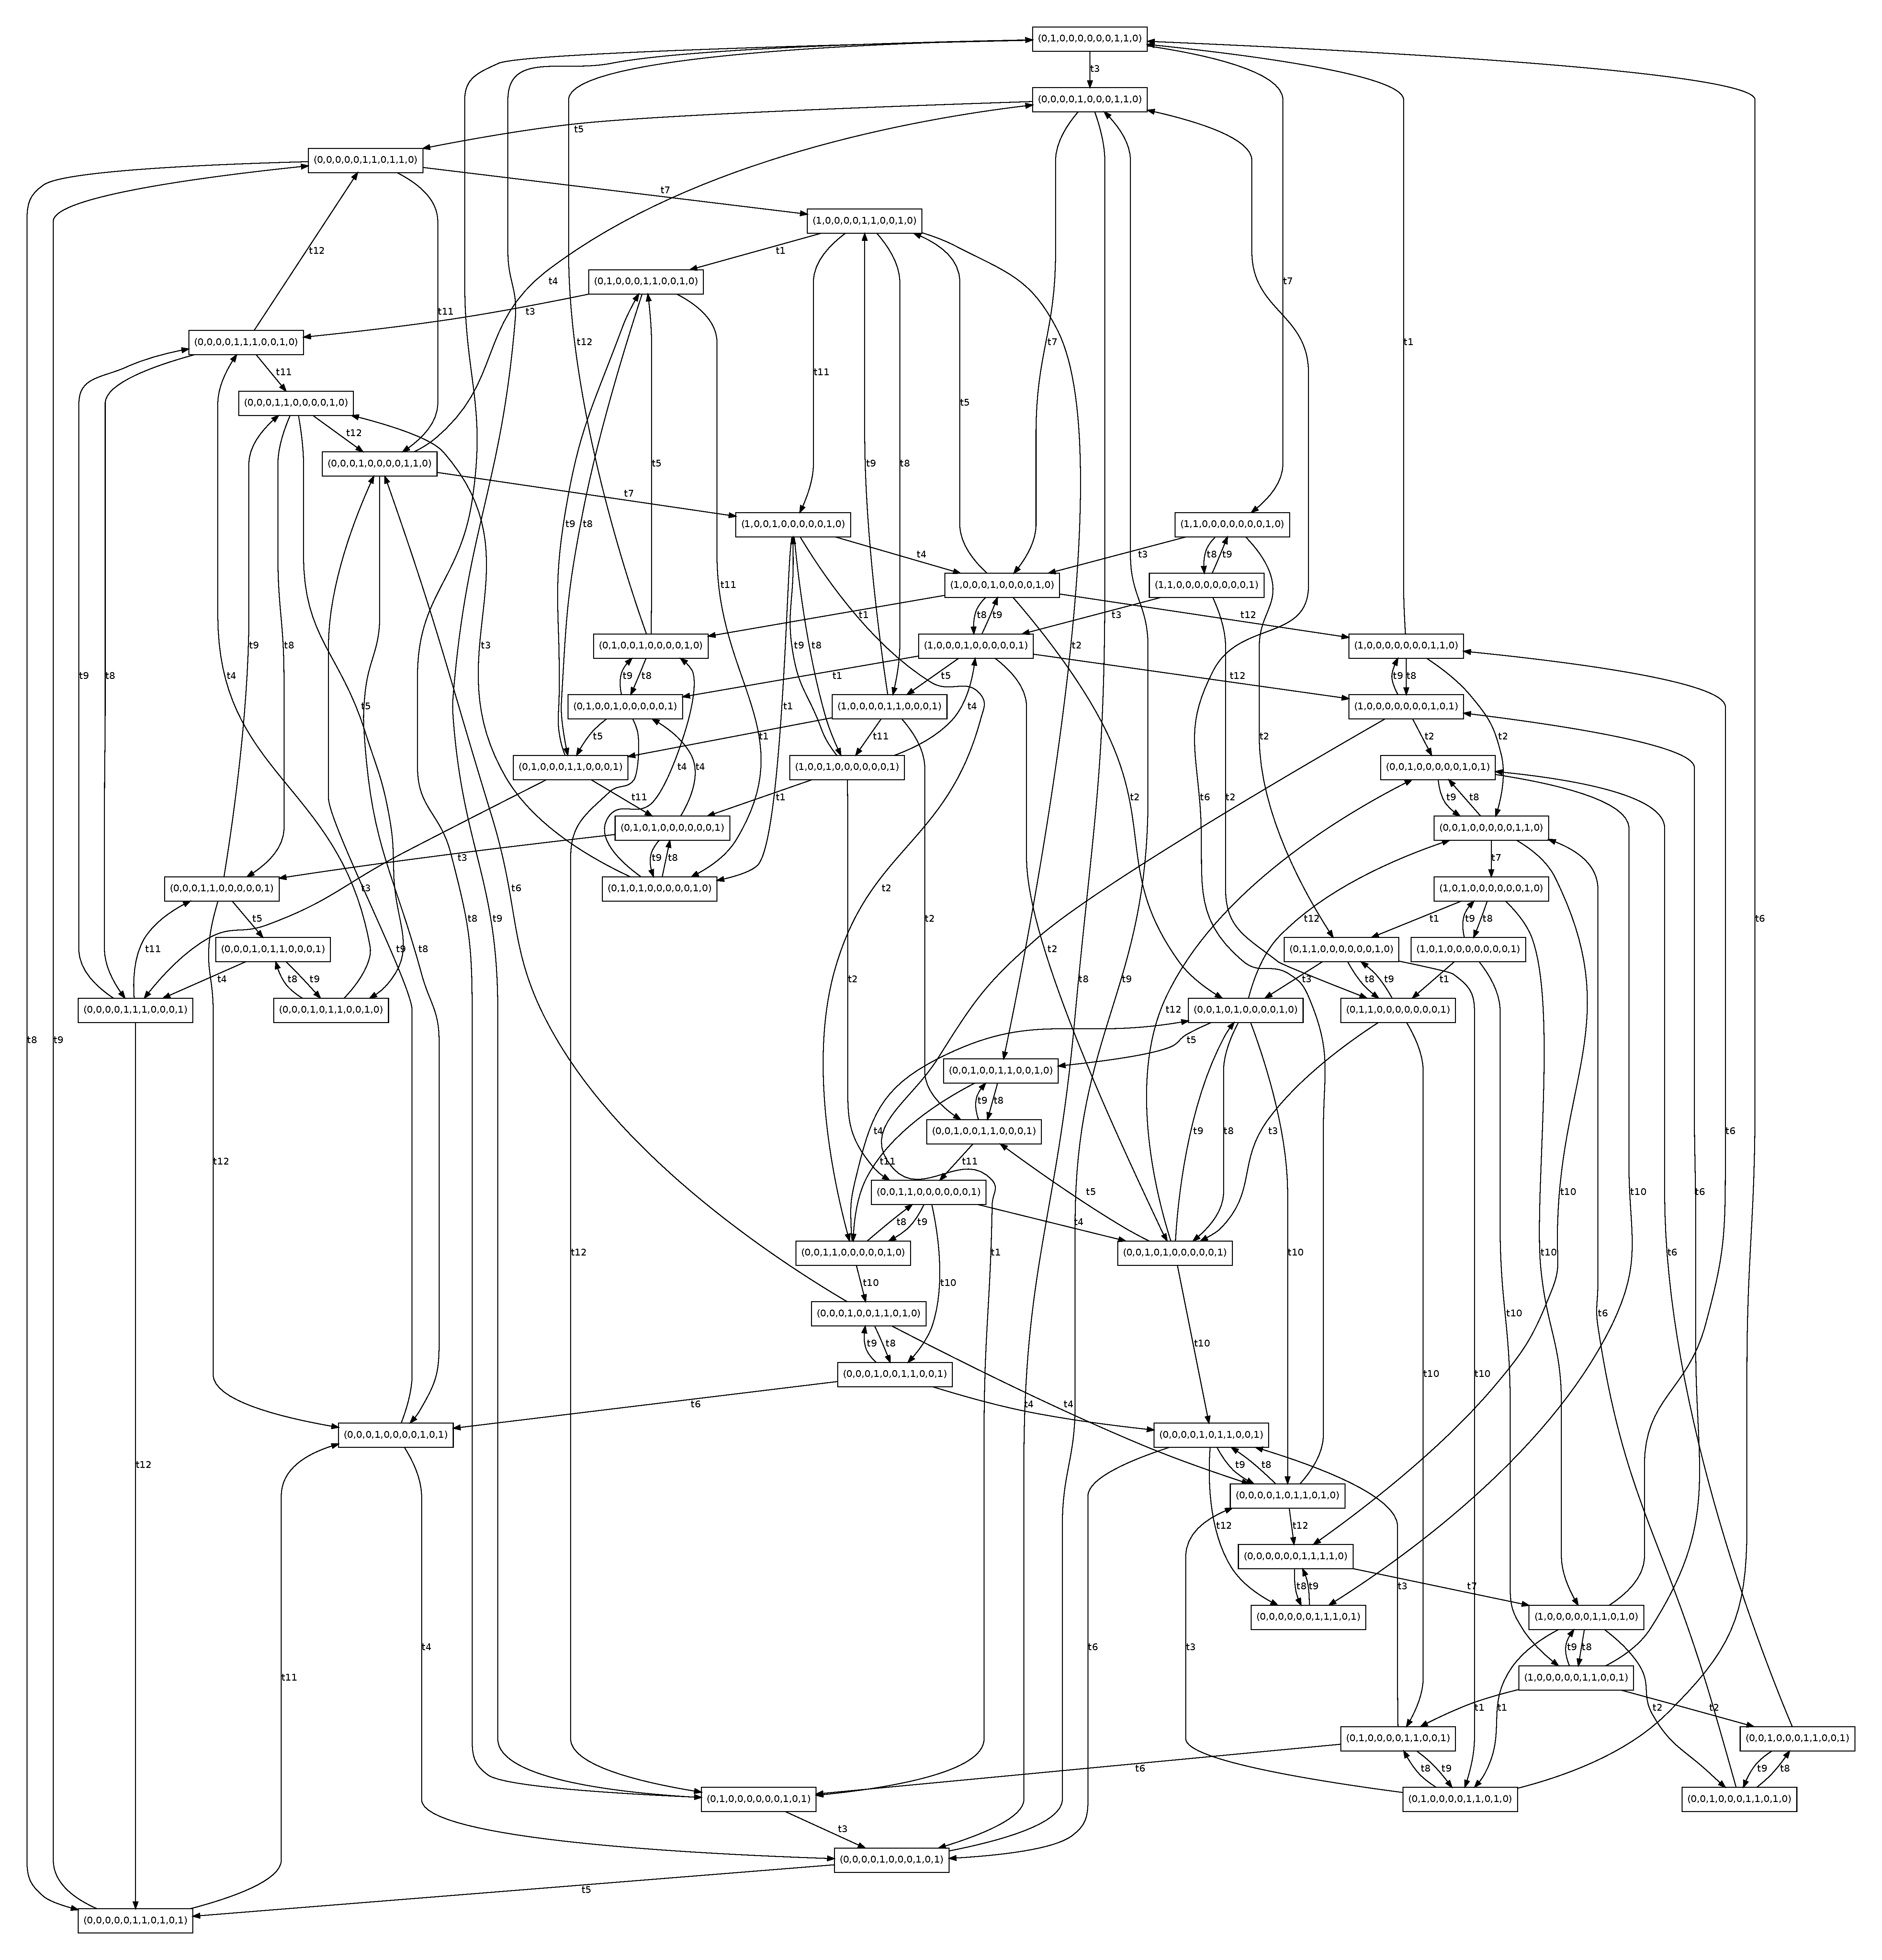
\includegraphics[width=1\textwidth]{eg.pdf}

Vereinfachte Version zur Berechnung der Kondensations- und Überdeckungsgraphen.

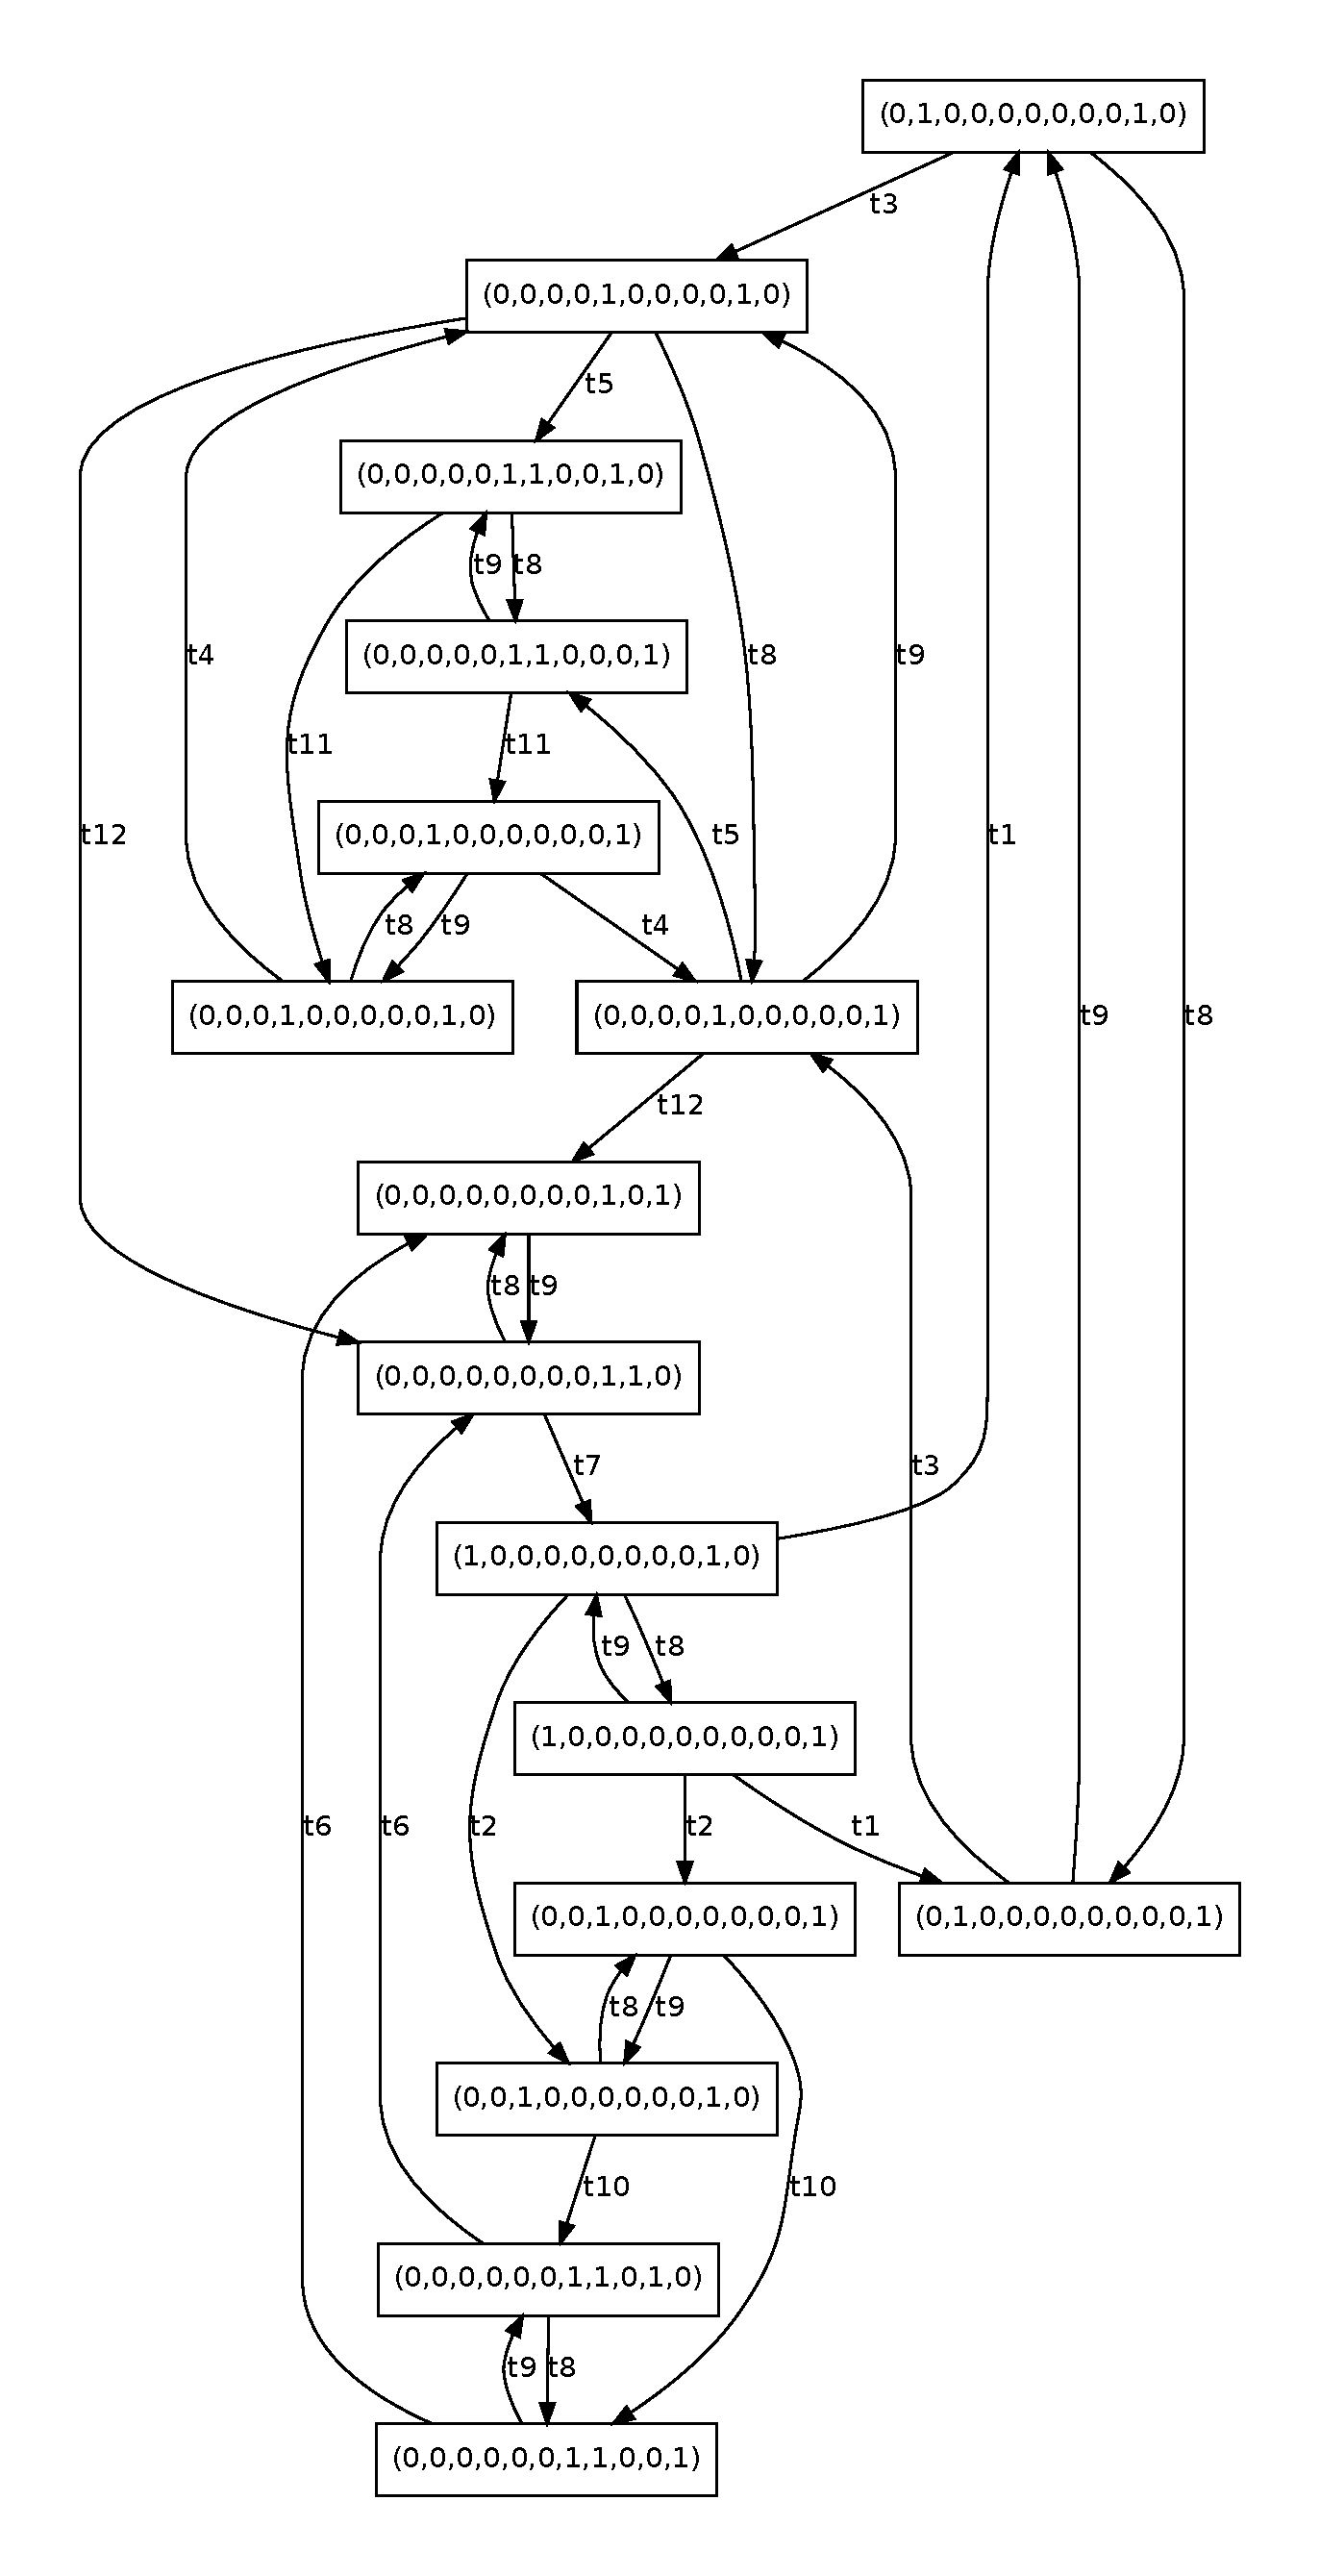
\includegraphics[width=0.9\textwidth]{eg_easy.pdf}

(d) Berechnet den Kondensationsgraph Eurer Gleisanlage.

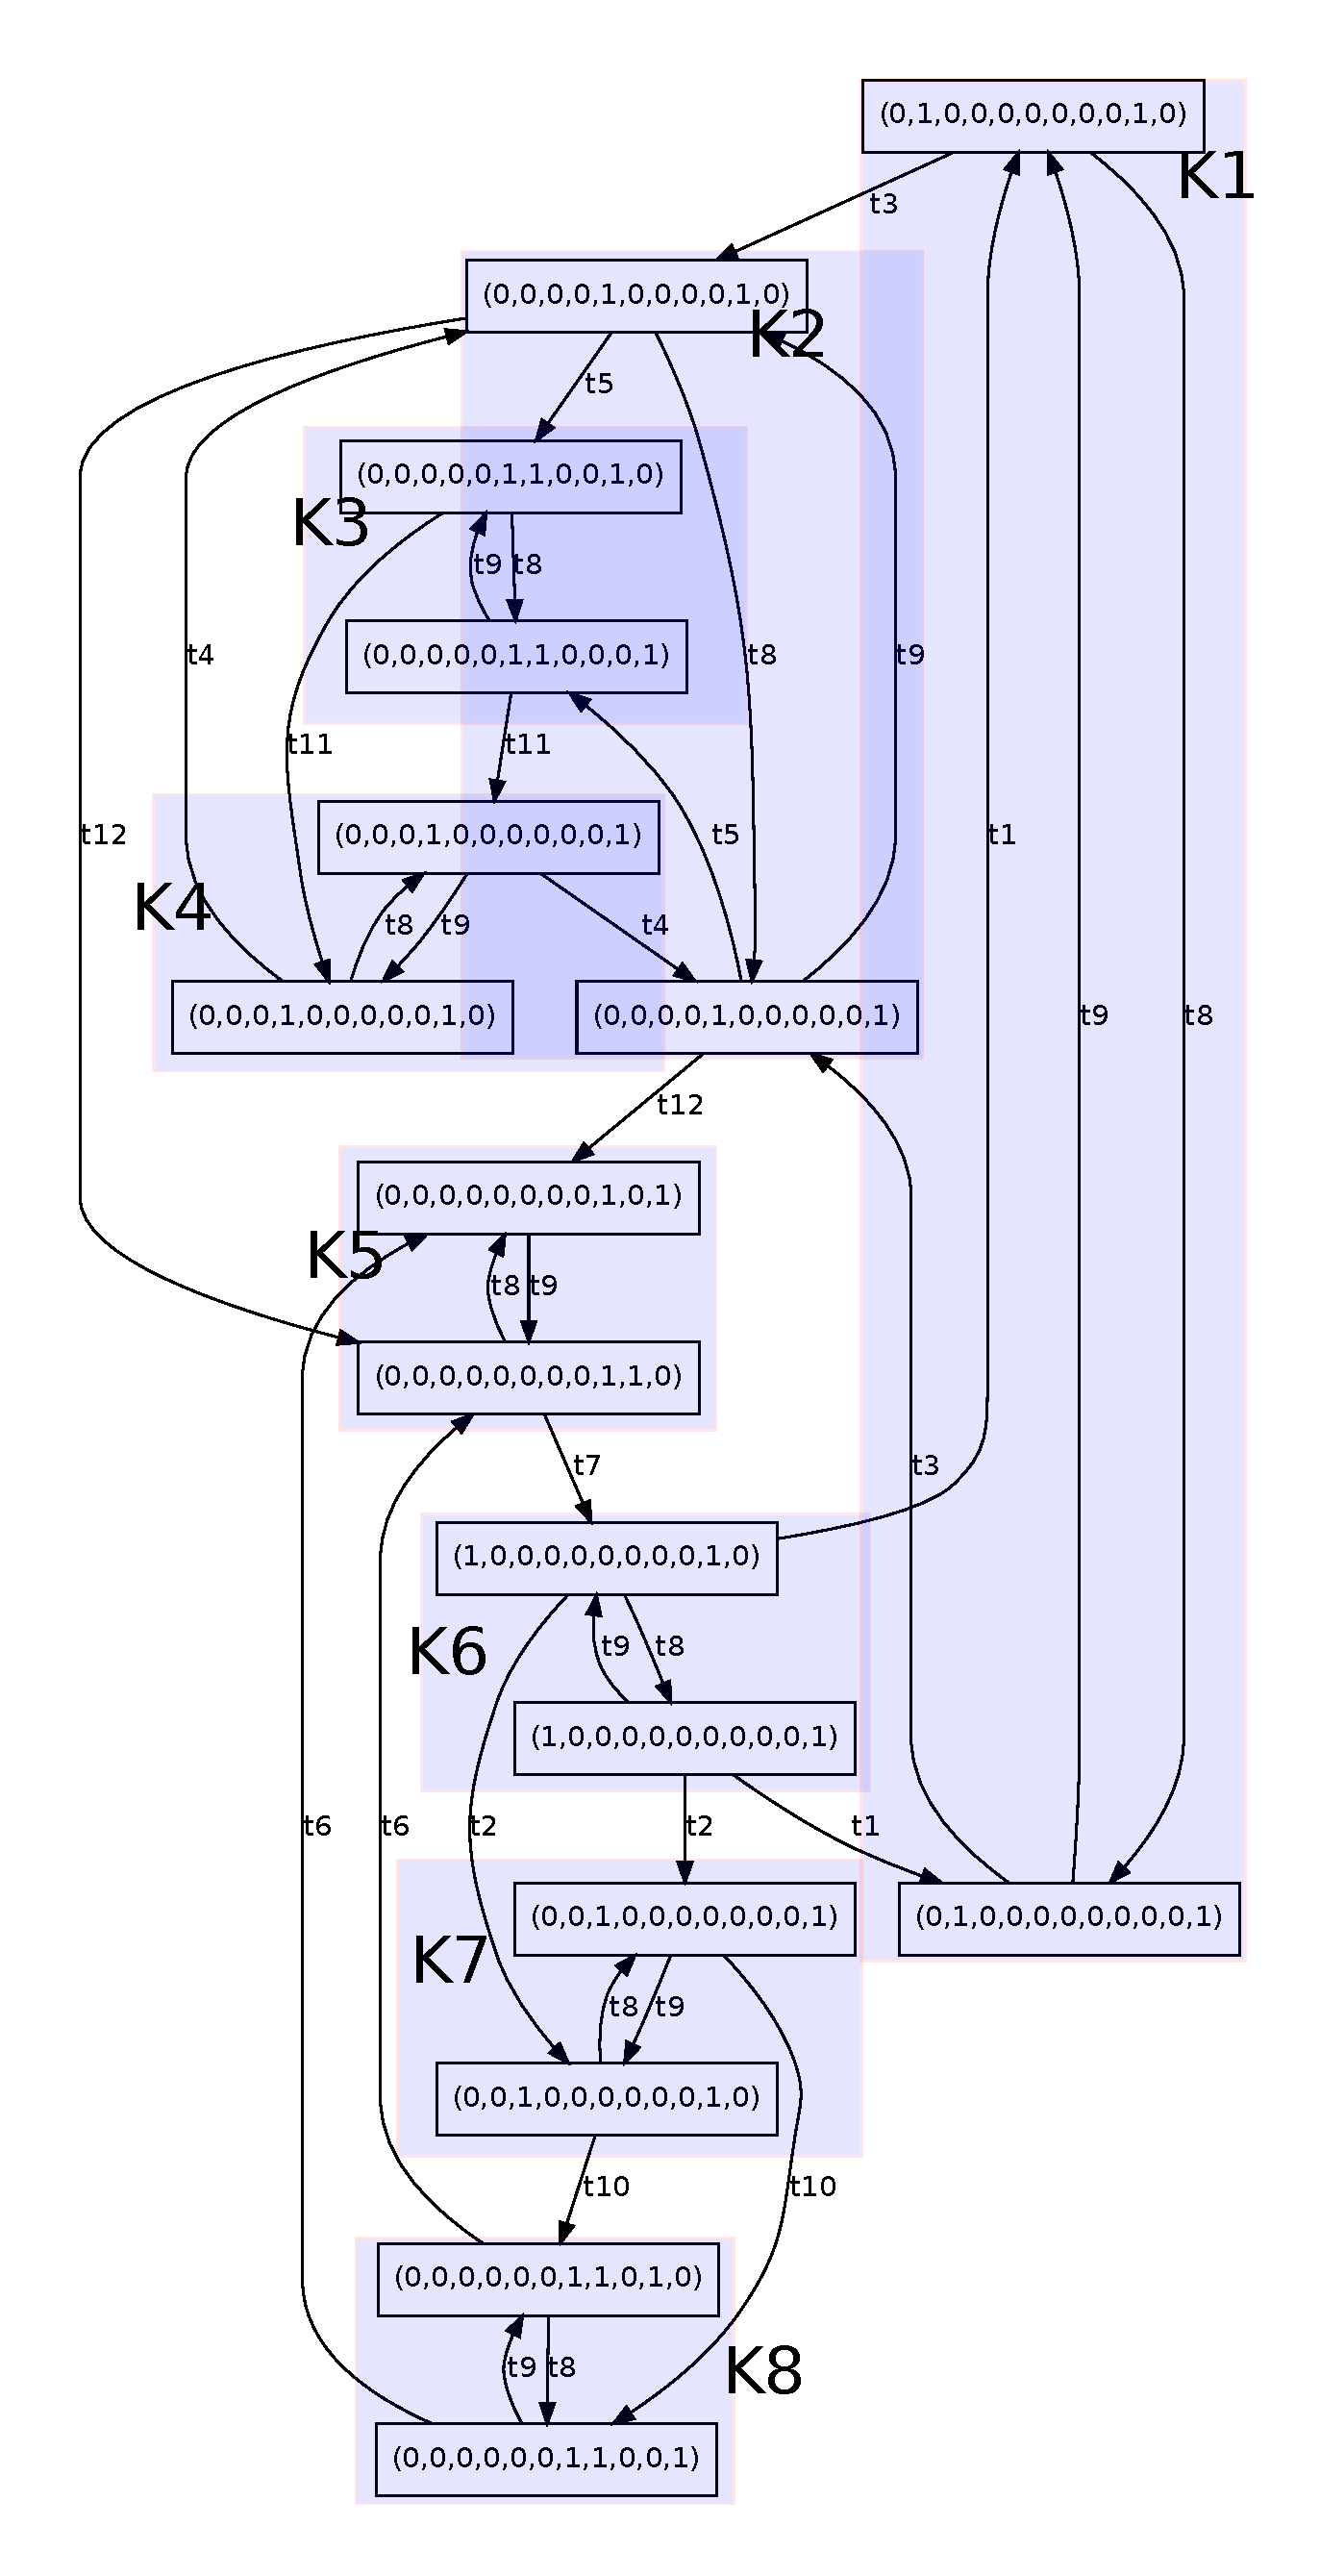
\includegraphics[width=0.7\textwidth]{kg_easy.pdf}

(e) Berechnet den Uberdeckungssgraph Eurer Gleisanlage.

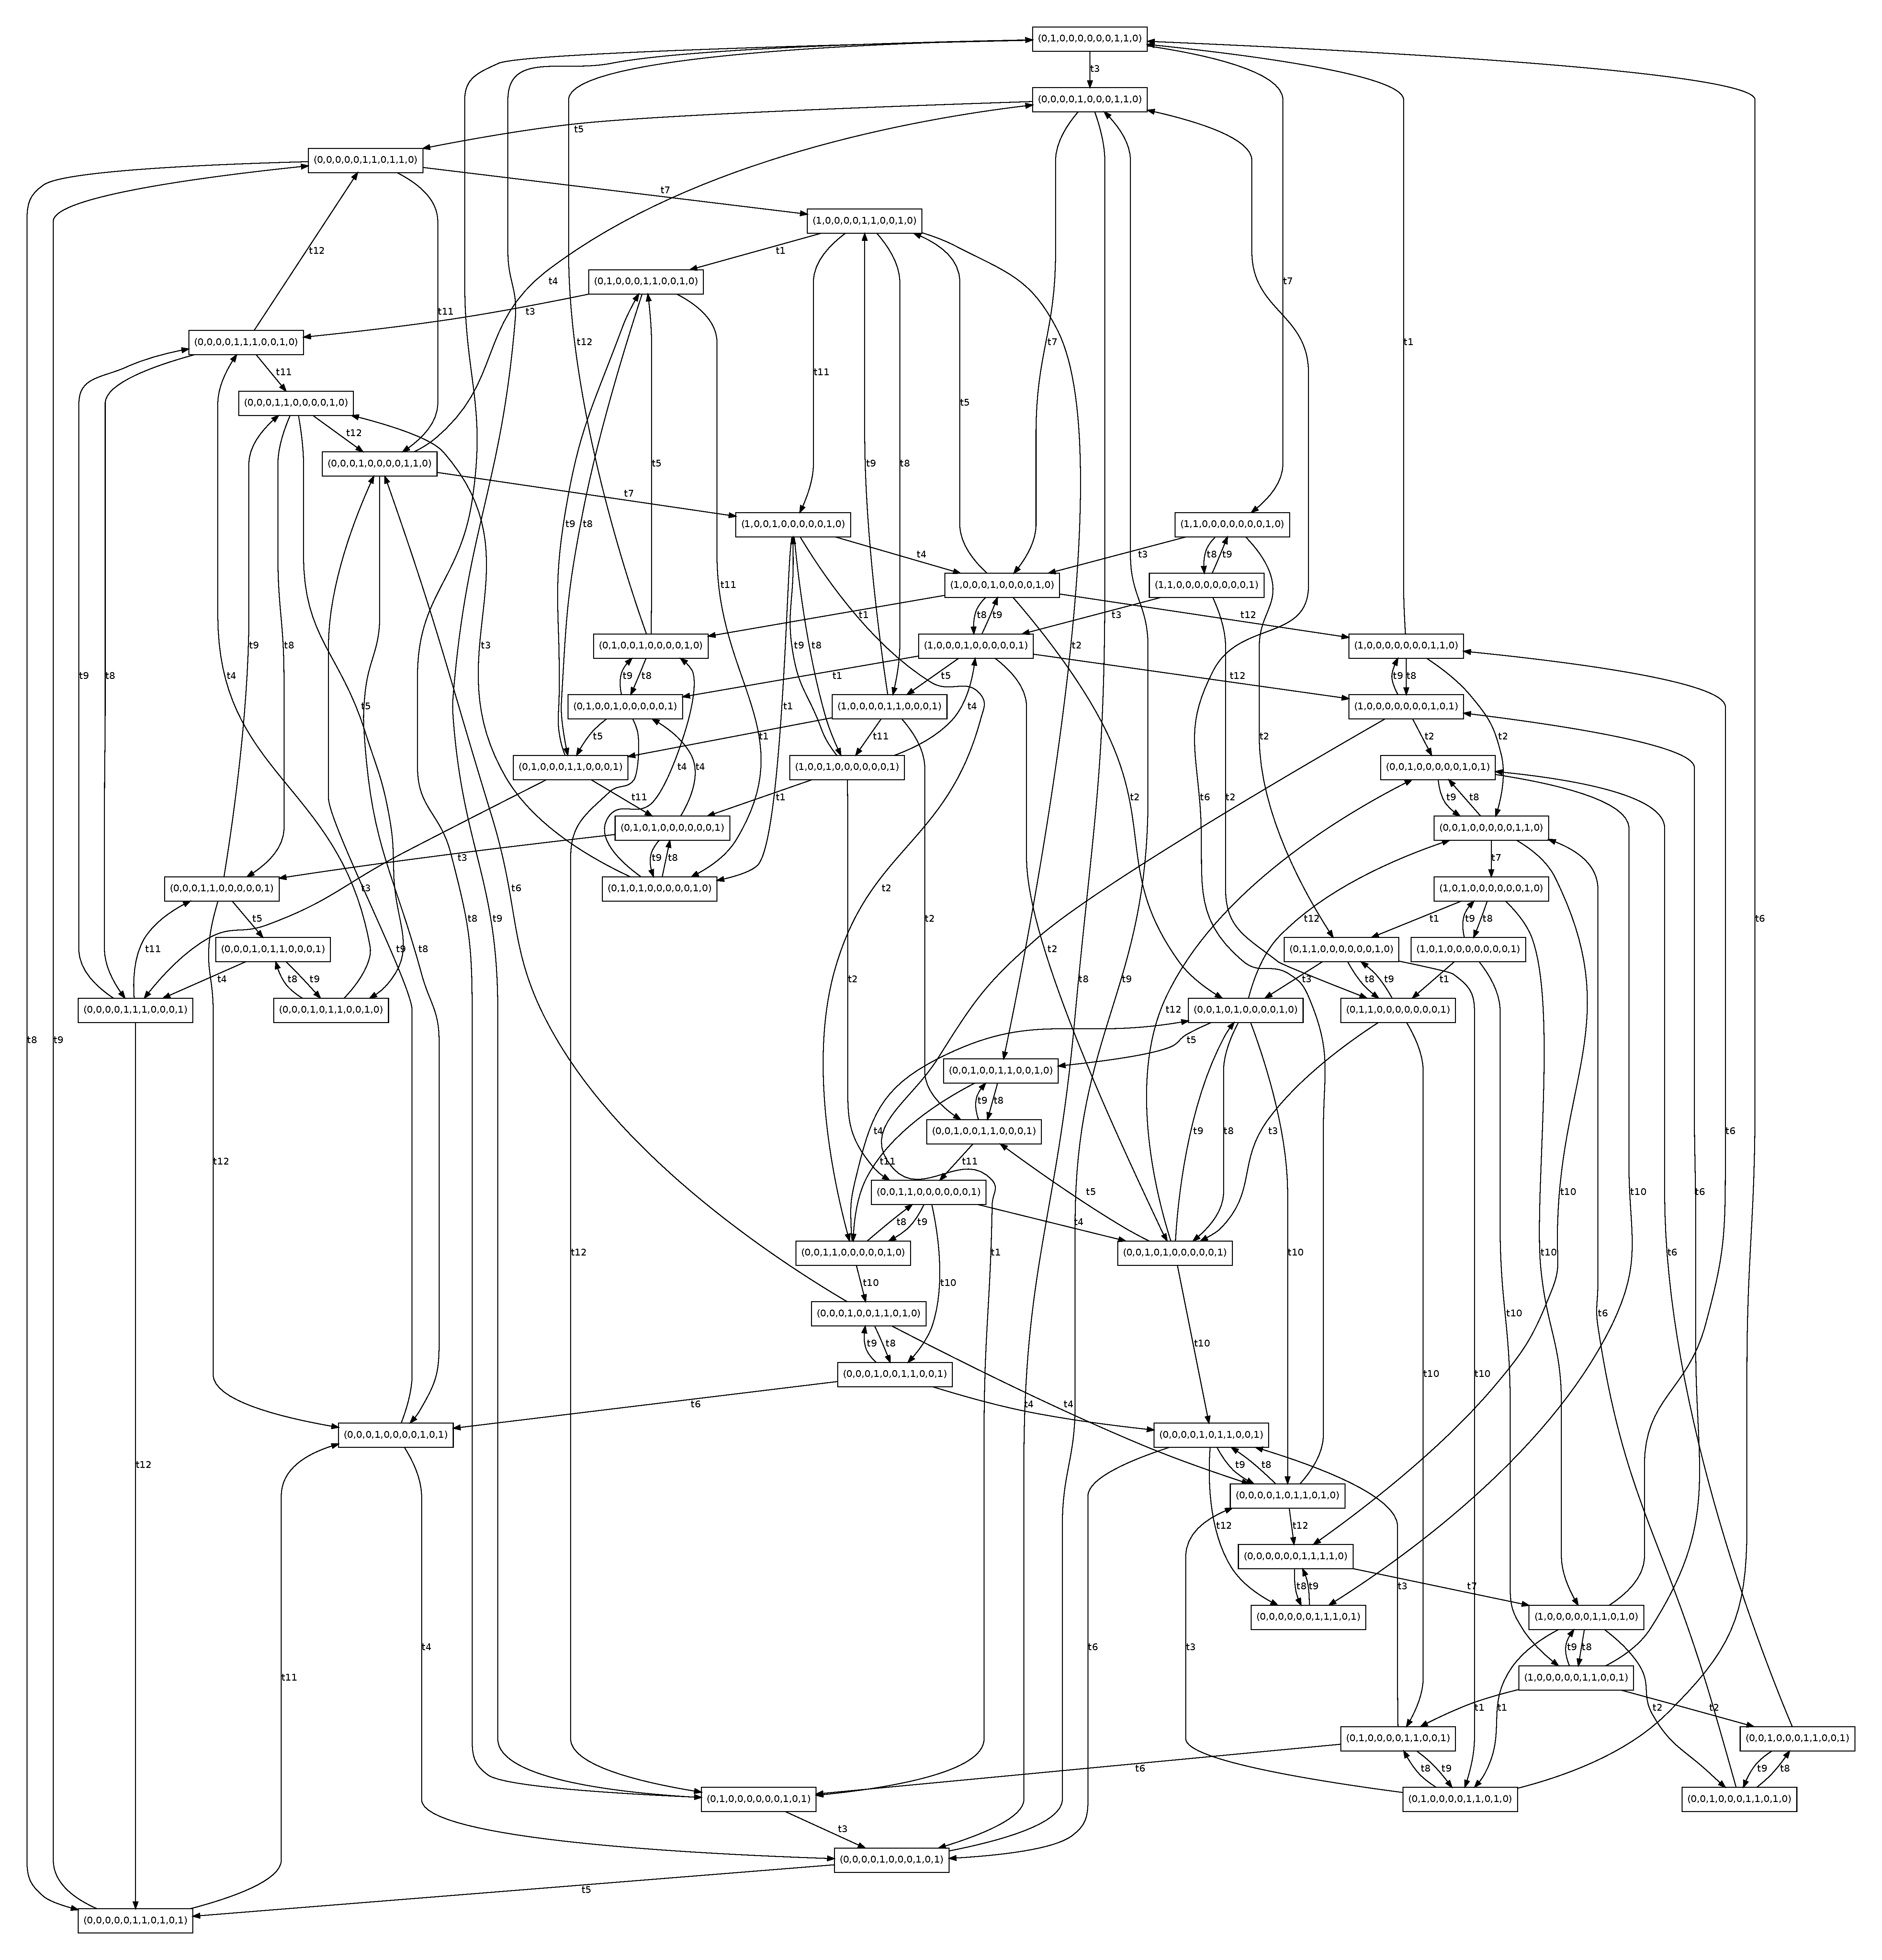
\includegraphics[width=1\textwidth]{eg.pdf}

\newpage

\item Verifikation:

(a) Welche Eigenschaften lassen sich aus den Invarianten und den Graphen für Eure Gleisanlage ablesen?

\textbf{Sicherheitseigenschaften:}

%\( P = \{LO, O, OML, OMR, R, MU, MG, MO, UL, SB, SF\} \)

Reversibilität (EG, kondensiert):
\textbf{Das Netz ist reversibel.}
Notwendige Bedingungen aus Invarianten:
  Es existiert eine nichtnegative T-Invariante.
  Damit ist die notwendige Bedingung für Reversibilität erfüllt,
  das Netz kann Reversibel sein.

$I_{P_1} = (1, 1, 1, 1, 1, 0, 1, 0, 1, 0, 0)^T$

Auf dem mittleren Streckenabschnitt können sich keine 2 Züge entgegenkommen (wechselseitiger Ausschluss), da $LO + O + OML + OMR + R + MG + UL = 2$. 

$I_{P_2} = (0, 0, 0, 0, 0, 0, 0, 0, 0, 1, 1)^T$

$SB + SF = 1 \implies$ Wechselseitiger Ausschluss von 'Bahnübergang offen' und 'Bahnübergang geschlossen'.

$I_{P_3} = (1, 1, 1, 1, 1, 1, 0, 1, 1, 0, 0)^T$

Nie mehr als 1 Zug auf einem Streckenabschnitt und es geht kein Zug verloren, da $LO + O + OML + OMR + R + MU + MO + UL = 2$

\textbf{Lebendigkeitseigenschaften:}

Reversibilität (EG, kondensiert):
\textbf{Das Netz ist reversibel.}
Notwendige Bedingungen aus Invarianten:
  Es existiert eine nichtnegative T-Invariante.
  Damit ist die notwendige Bedingung für Reversibilität erfüllt,
  das Netz kann Reversibel sein.

Lebendigkeit (EG, kondensiert):
\textbf{Das Netz ist lebendig.}
Notwendige Bedingungen aus Invarianten:
  Es existiert eine positive T-Invariante.
  Damit ist die notwendige Bedingung für Lebendigkeit erfüllt,
  das Netz kann lebendig sein.

%           T1 T2 T3 T4 T5 T6 T7 T8 T9 10 11 12

$I_{T_1} = (0, 0, 0, 0, 0, 0, 0, 1, 1, 0, 0, 0)$

Vollständiger Prozess: Bahnübergang schließen, Bahnübergang öffnen, d.h. wechselnd.

$I_{T_2} = (0, 1, 0, 0, 0, 1, 1, 0, 0, 1, 0, 0)$

Vollständiger Prozess: kleine, linke Runde fahren.

$I_{T_3} = (0, 0, 0, 1, 1, 0, 0, 0, 0, 0, 1, 0)$

Vollständiger Prozess: kleine, rechte Runde fahren.

$I_{T_4} = (1, 0, 1, 0, 0, 0, 1, 0, 0, 0, 0, 1)$

Vollständiger Prozess: große Runde fahren.

(b) Inwiefern ändern sich die Ergebnisse, wenn nur ein Zug fährt oder mehr als zwei Züge fahren. Gelten die Eigenschaften dann in jedem Fall immer noch?

a) Fährt nur noch ein Zug, ändern sich die Eigenschaften des Netzes nicht. 

Es ist lediglich eine Stelle weniger belegt und damit pro Markierung eine oder zwei Transistionen weniger aktiviert. Überdeckungs- und Kondensationsgraph werden damit kleiner.

% TODO ^ Überdeckungs- & Kondensationsgraph berechnen und malen? Morgen nach der Klausur? ;-)

b) Fahren mehr als 2 Züge, lautet die maximale ``gültige'' Startmarkierung

\( M_0 = \begin{pmatrix}
1 \\ % LO
1 \\ % O
1 \\ % OML
1 \\ % OMR
1 \\ % R
1 \\ % MU
1 \\ % MG
0 \\ % MO
1 \\ % UL
0 \\ % SB
1 \\ % SF
\end{pmatrix} \)

Erhalten die verbleibenden Stellen auch eine Markierung, sind aufgrund der Kapazitäten keine Transitionen mehr aktiviert. Damit verliert das Netz seine Lebendigkeitseigenschaft.

% TODO 

(c) Lassen sich alle Eure gewünschten Eigenschaften aus 1. mit Hilfe der Analyse verifizieren? Wenn ja, dann formalisiert Eure gewünschten Eigenschaften und weist sie mithilfe der Analyse nach. Wenn nein, dann formuliert informell, warum sie nicht nachgewiesen werden können.

% TODO

\end{enumerate}

\end{document}

% vim: fileencoding=utf8
